\section{FaBoのブリックについて}
\subsection{FaBoの使い方}
今日の授業ではFaBoのシールドとFaBoのブリックを使います。この二つは簡単にセンサーとRaspberry Piとつなげるようにあらかじめ配線がされているものです。

\begin{figure}[htbp]
  \begin{minipage}[b]{0.45\linewidth}
    \centering
    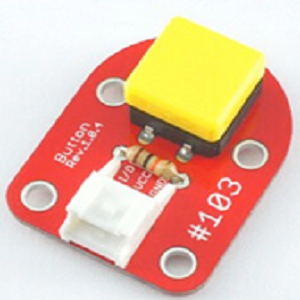
\includegraphics[keepaspectratio, scale=0.6]{images/chap05/text05-img028.png}
    \caption{デジタル信号の例}
    \label{fig4}
  \end{minipage}
  \begin{minipage}[b]{0.45\linewidth}
    \centering
    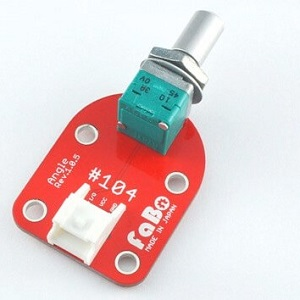
\includegraphics[keepaspectratio, scale=0.6]{images/chap05/text05-img022.jpg}
    \caption{アナログ信号の例}
    \label{fig5}
  \end{minipage}
\end{figure}

豆電球が電池で動くように、ブリックはRaspberry Piが電源となって動きます。本当ならばブリックとRaspberry Piをプラスマイナス、ブリックの出力などを考えて繋がないといけません。しかし、FaBoのシールドとブリックは必要な配線がすでにされているため、自分でどのように線を繋ぐかを考えなくても簡単に使えます。
それでは、さっそくFaBoをつかってみましょう。\\

{\Large\textcolor{red}{注意!}}\\
FaboのシールドをRaspberry Piとつなげるときは、必ずRaspberry Piをシャットダウンして電源を切りましょう。\\
\\
\begin{enumerate}
\item Raspberry Piの電源を切ります。\\
\item FaBoのシールドをRaspberry Piとつなげます。この時、なるべくシールドをまっすぐに押しこむようにしましょう。ピン(金属の棒の部分)を曲げないように注意してください。シールドにもトゲのある所があるのでケガをしないように注意しましょう。\\
\begin{figure}[H]
 \centering
 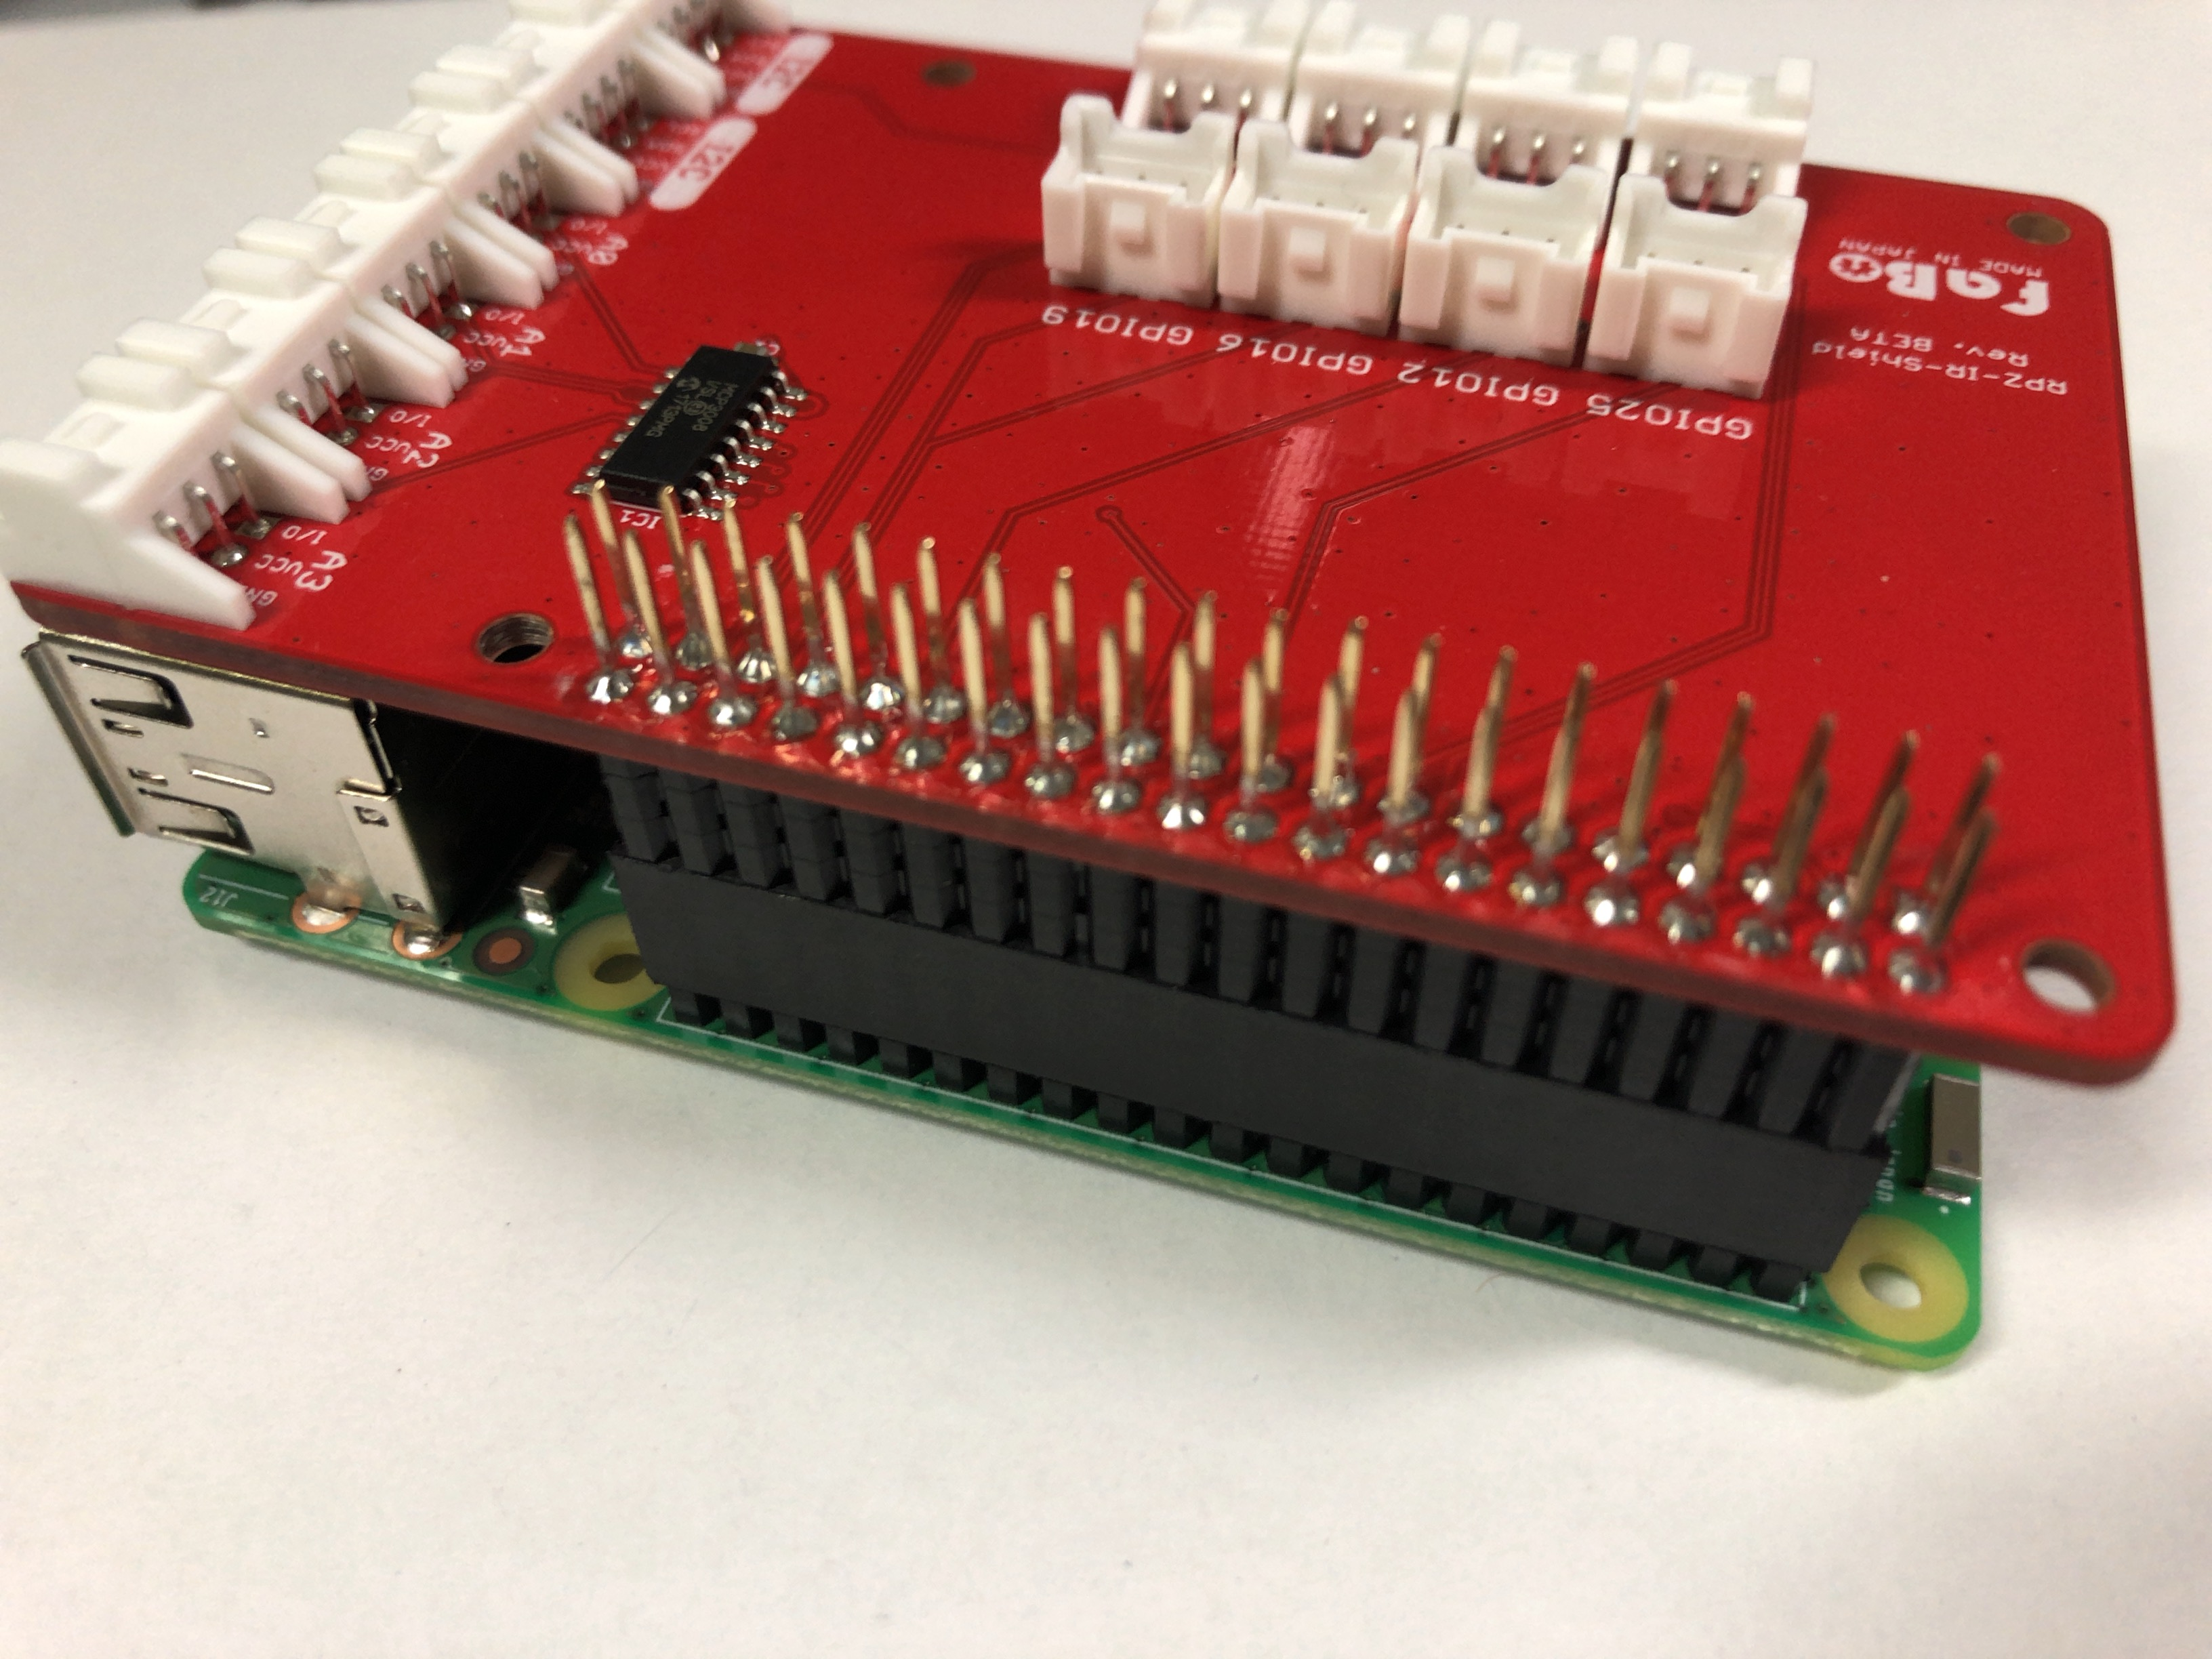
\includegraphics[width=\hsize/2]{images/chap05/text05-img006.jpg}
 \caption{FaBoのシールドとRaspberry Piのせつぞく}
\end{figure}
\item 同様にして、センサーボードをFaBoのシールドの上につなげます。\\
\begin{figure}[H]
 \centering
 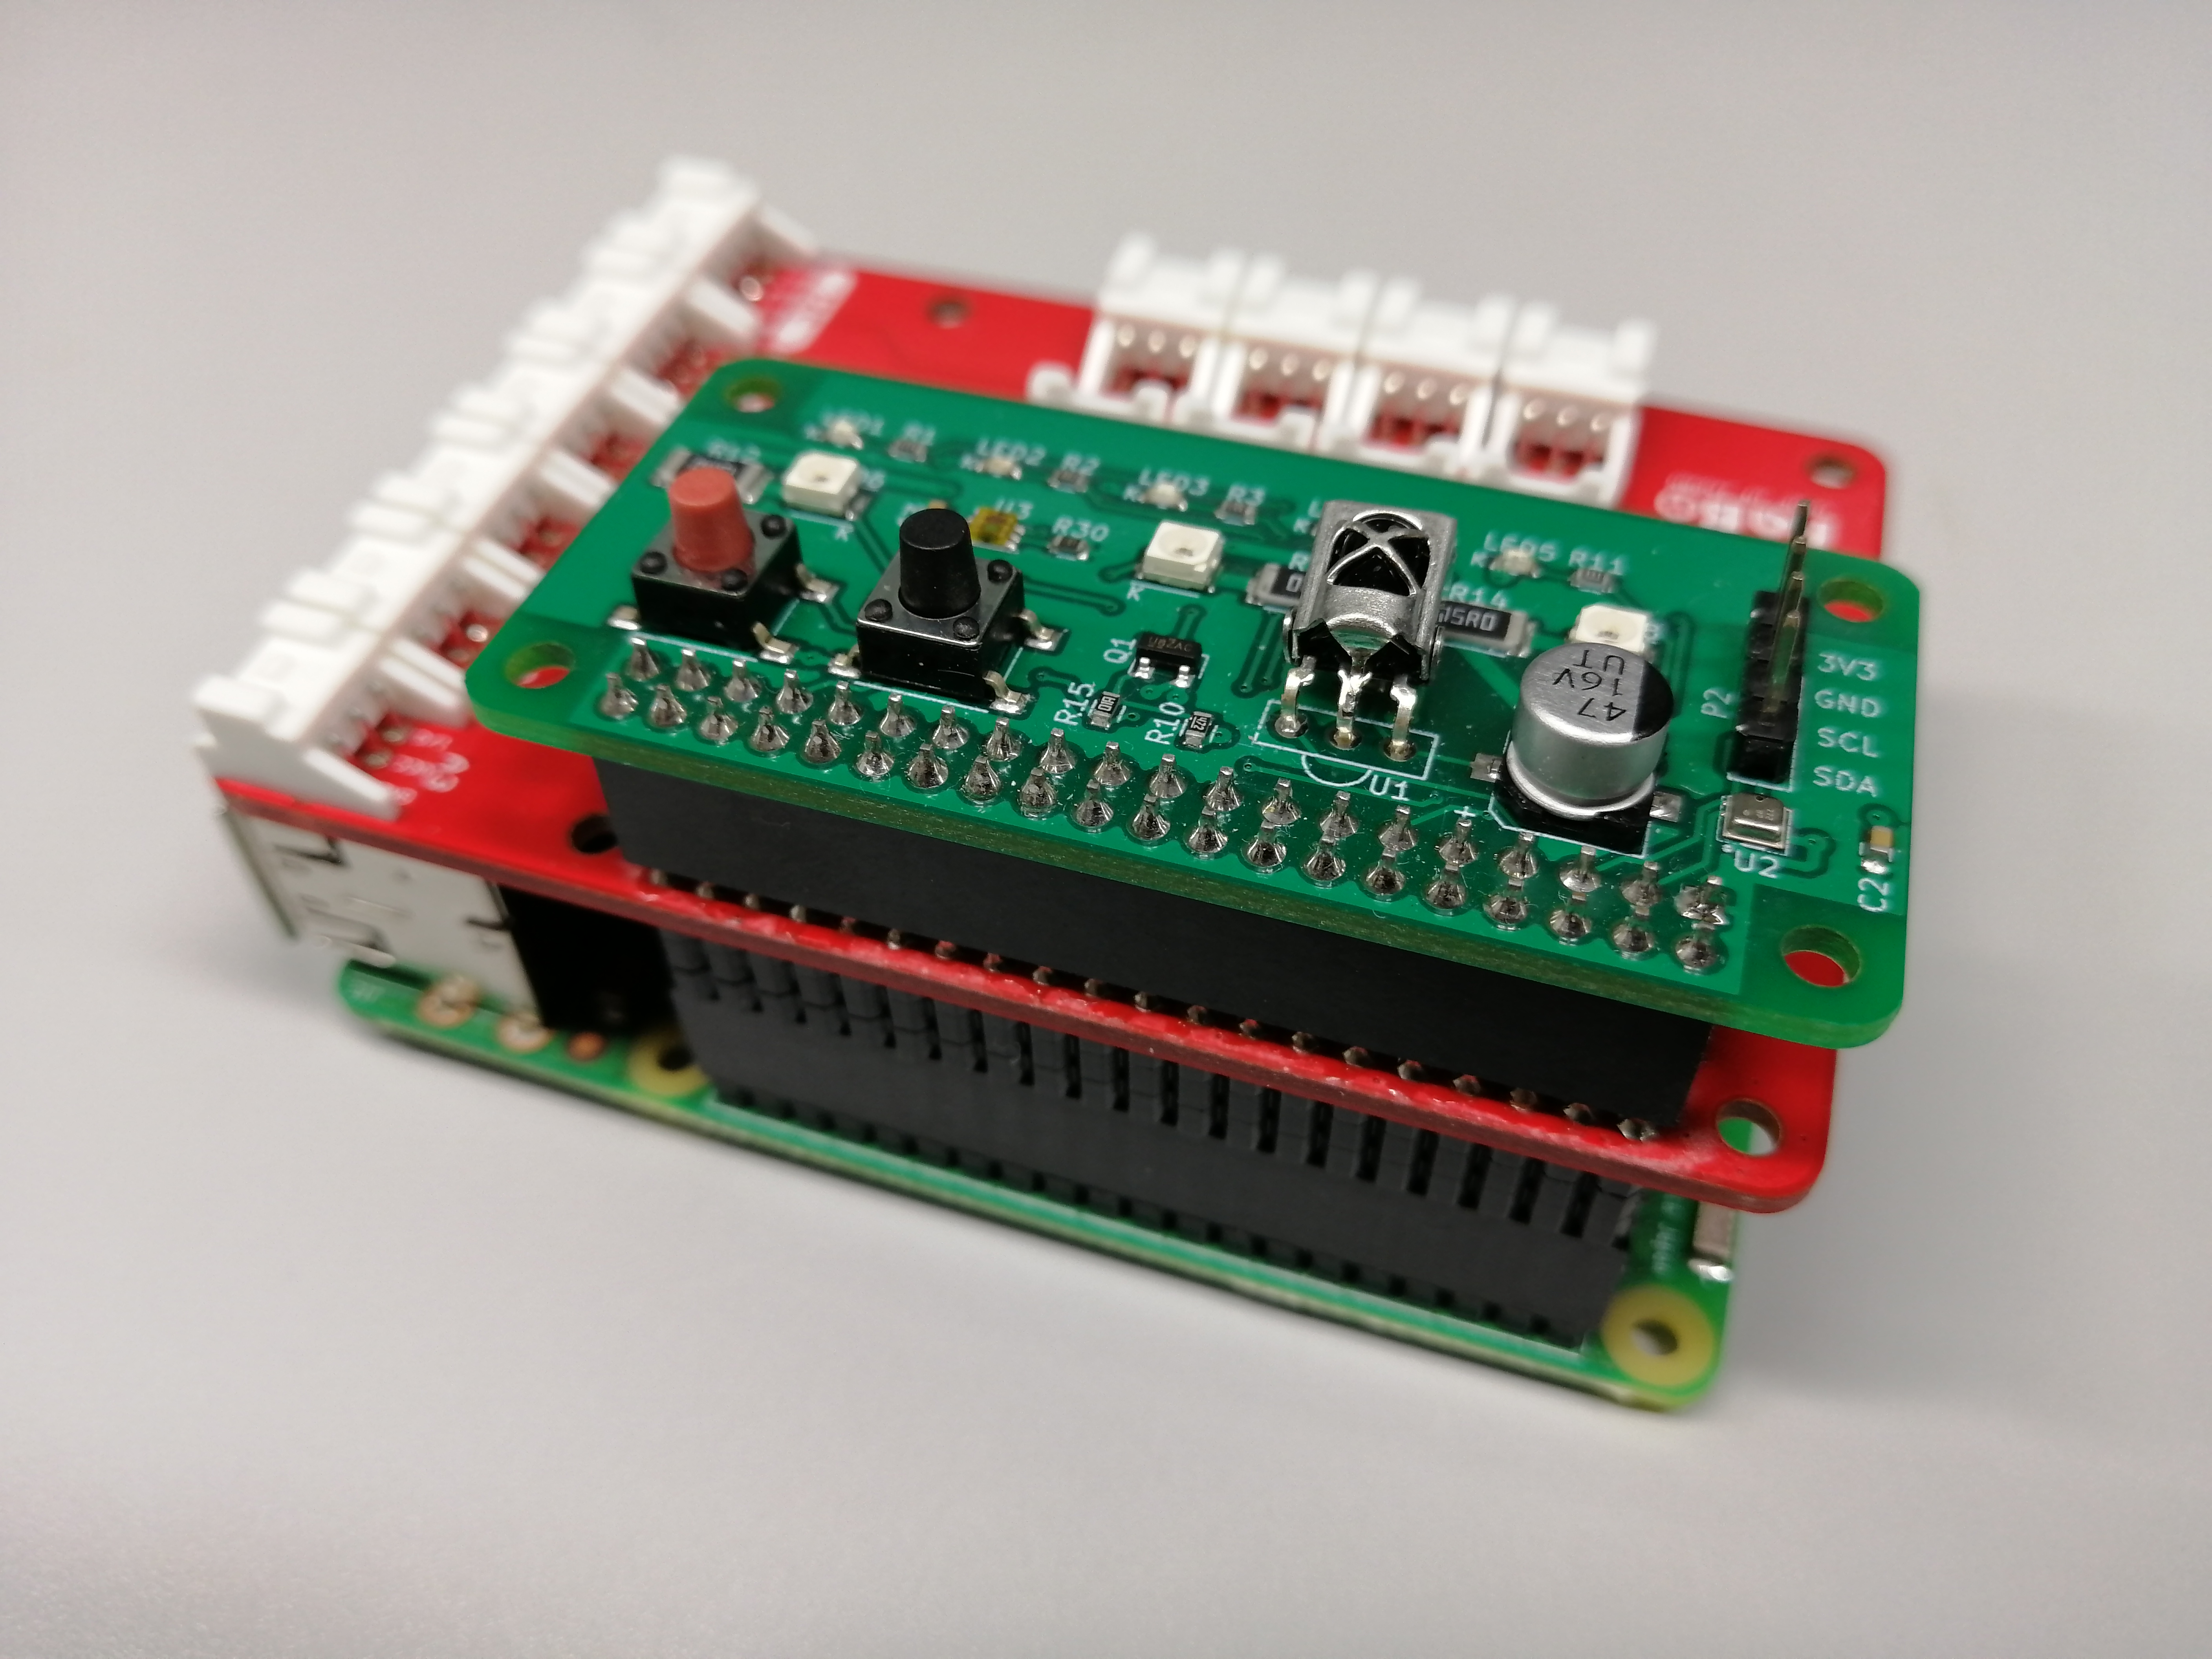
\includegraphics[width=\hsize/2]{images/chap05/text05-img007.jpg}
 \caption{センサーボードとFaBoのシールドのせつぞく}
\end{figure}
\item LEDをケーブルとつなげましょう。奥までケーブルを押しこんでください。\\
\begin{figure}[H]
 \centering
 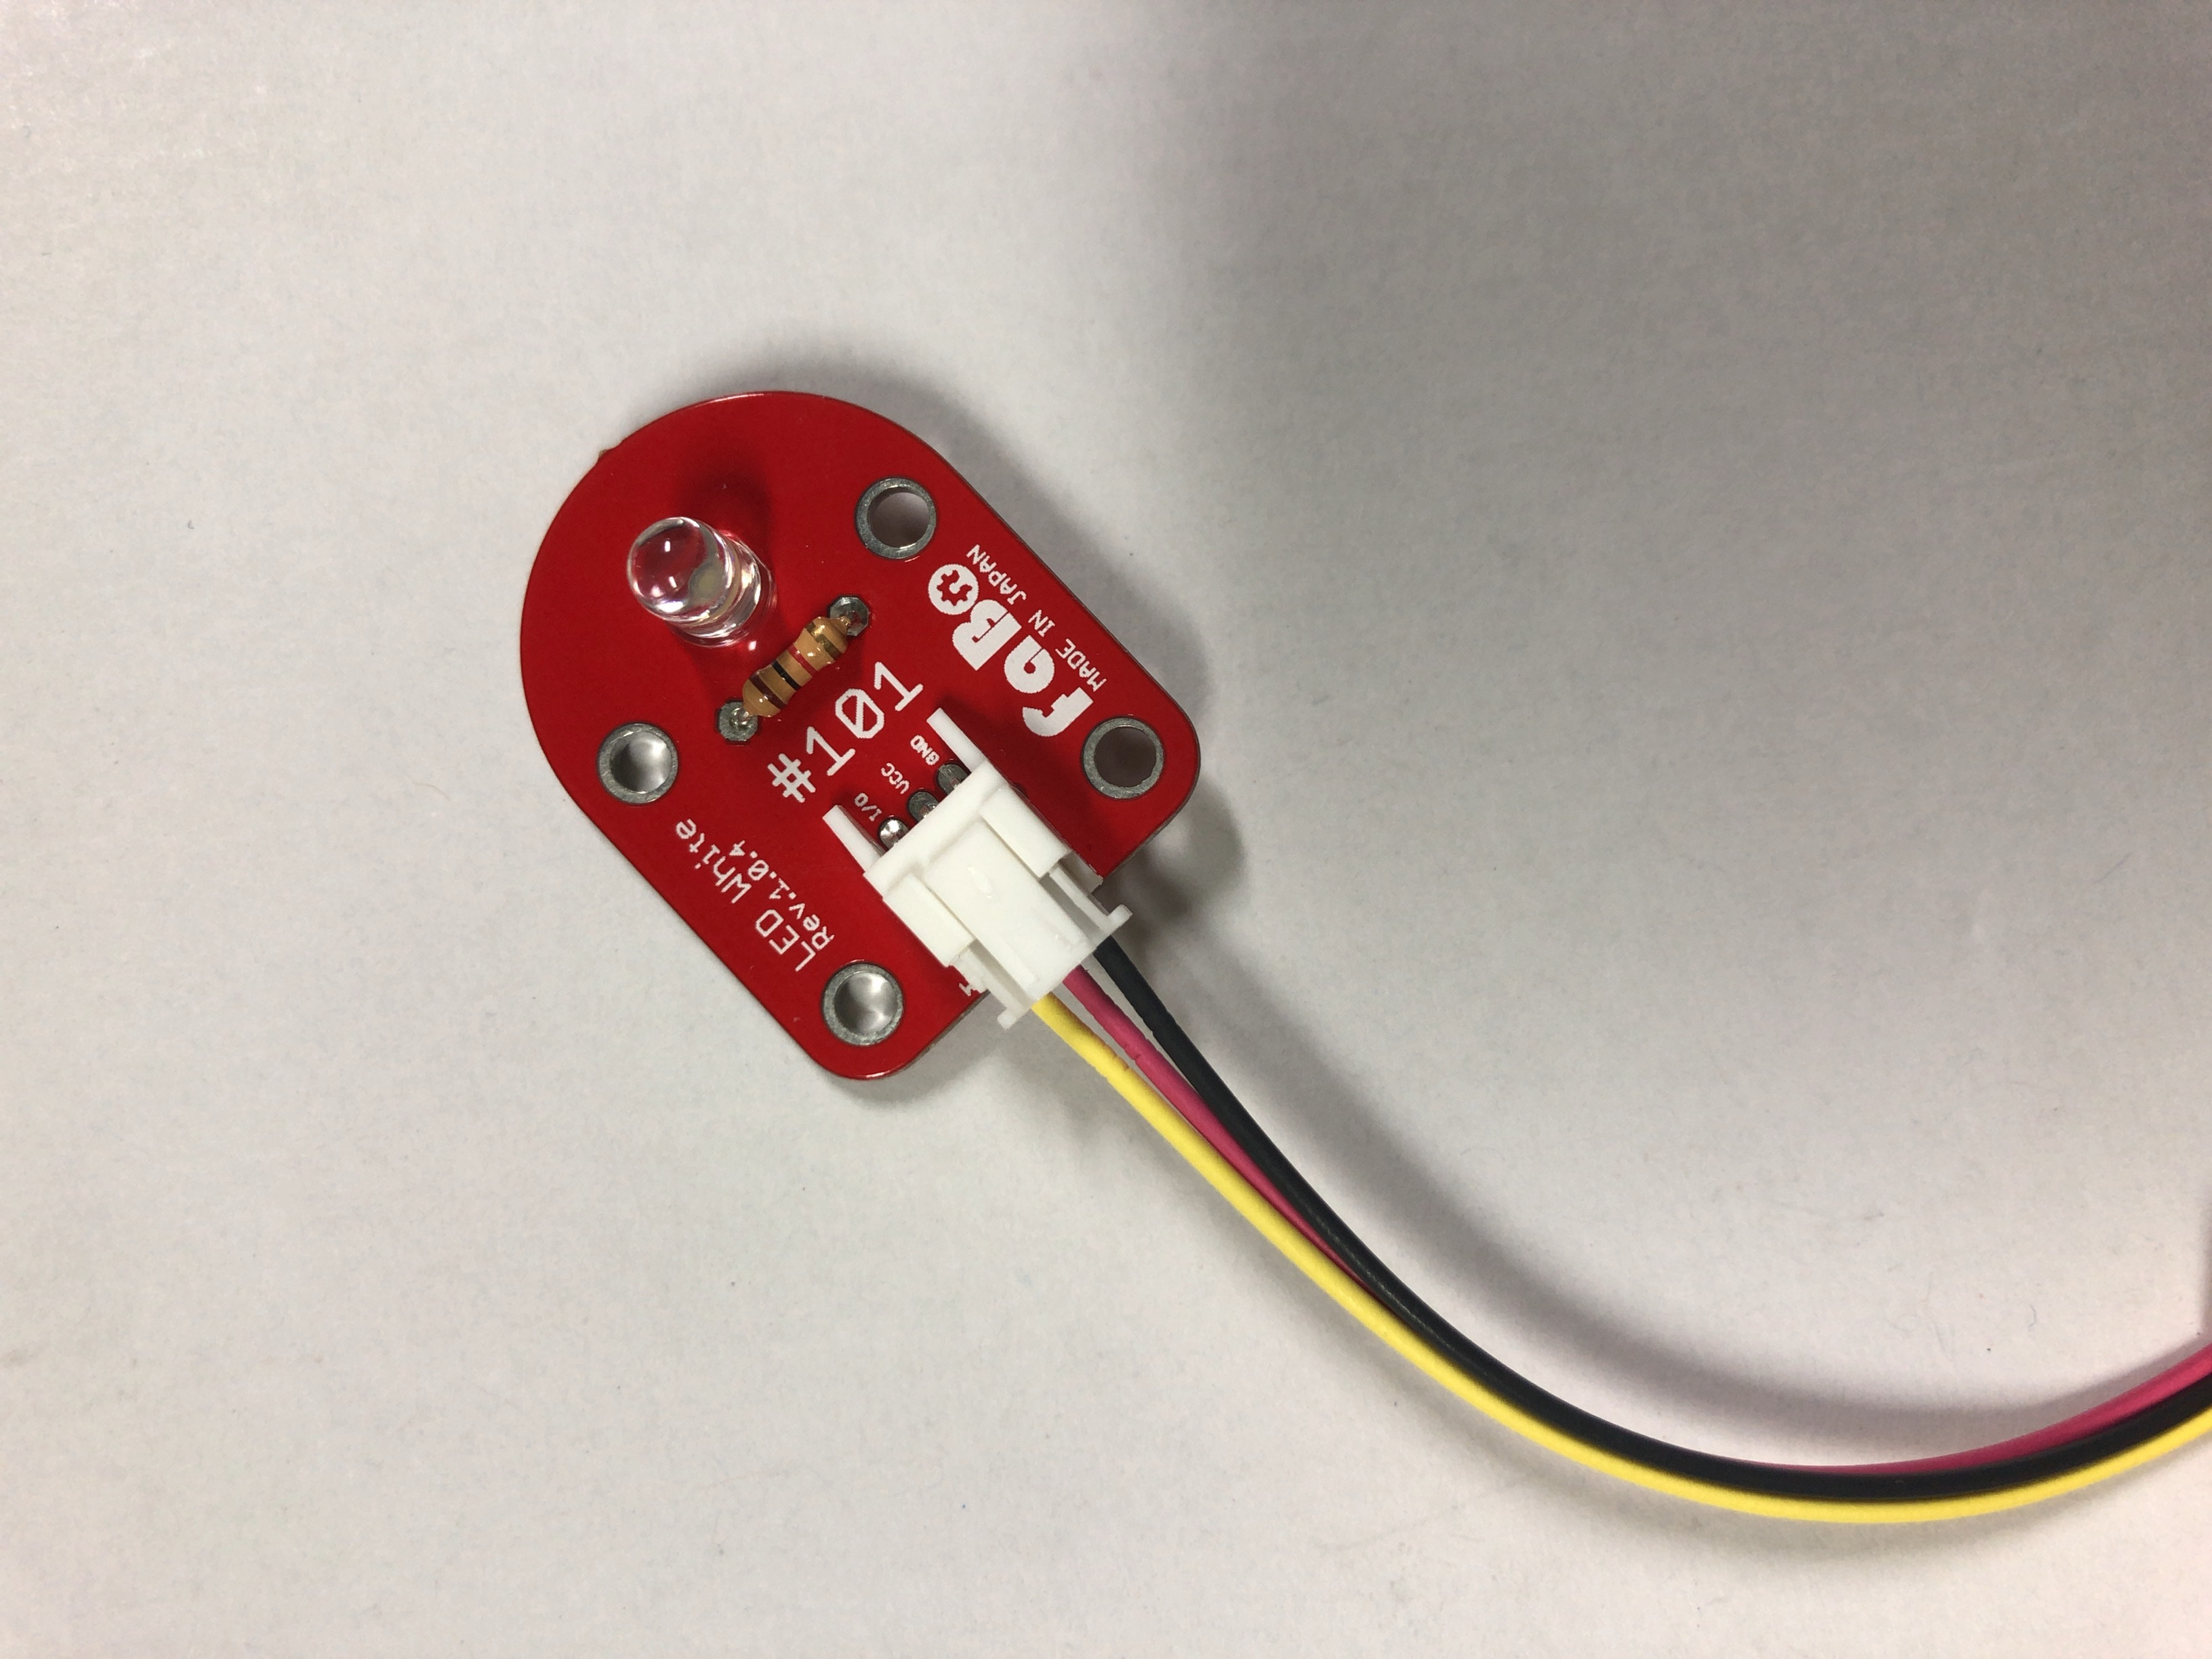
\includegraphics[width=\hsize/2]{images/chap05/text05-img008.jpg}
 \caption{Faboのブリックとケーブルのせつぞく}
\end{figure}
\item シールドとケーブルをつなげましょう。今回はGPIO23のところにつなげます。このときも奥までケーブルを押しこんでください。\\
\begin{figure}[H]
 \centering
 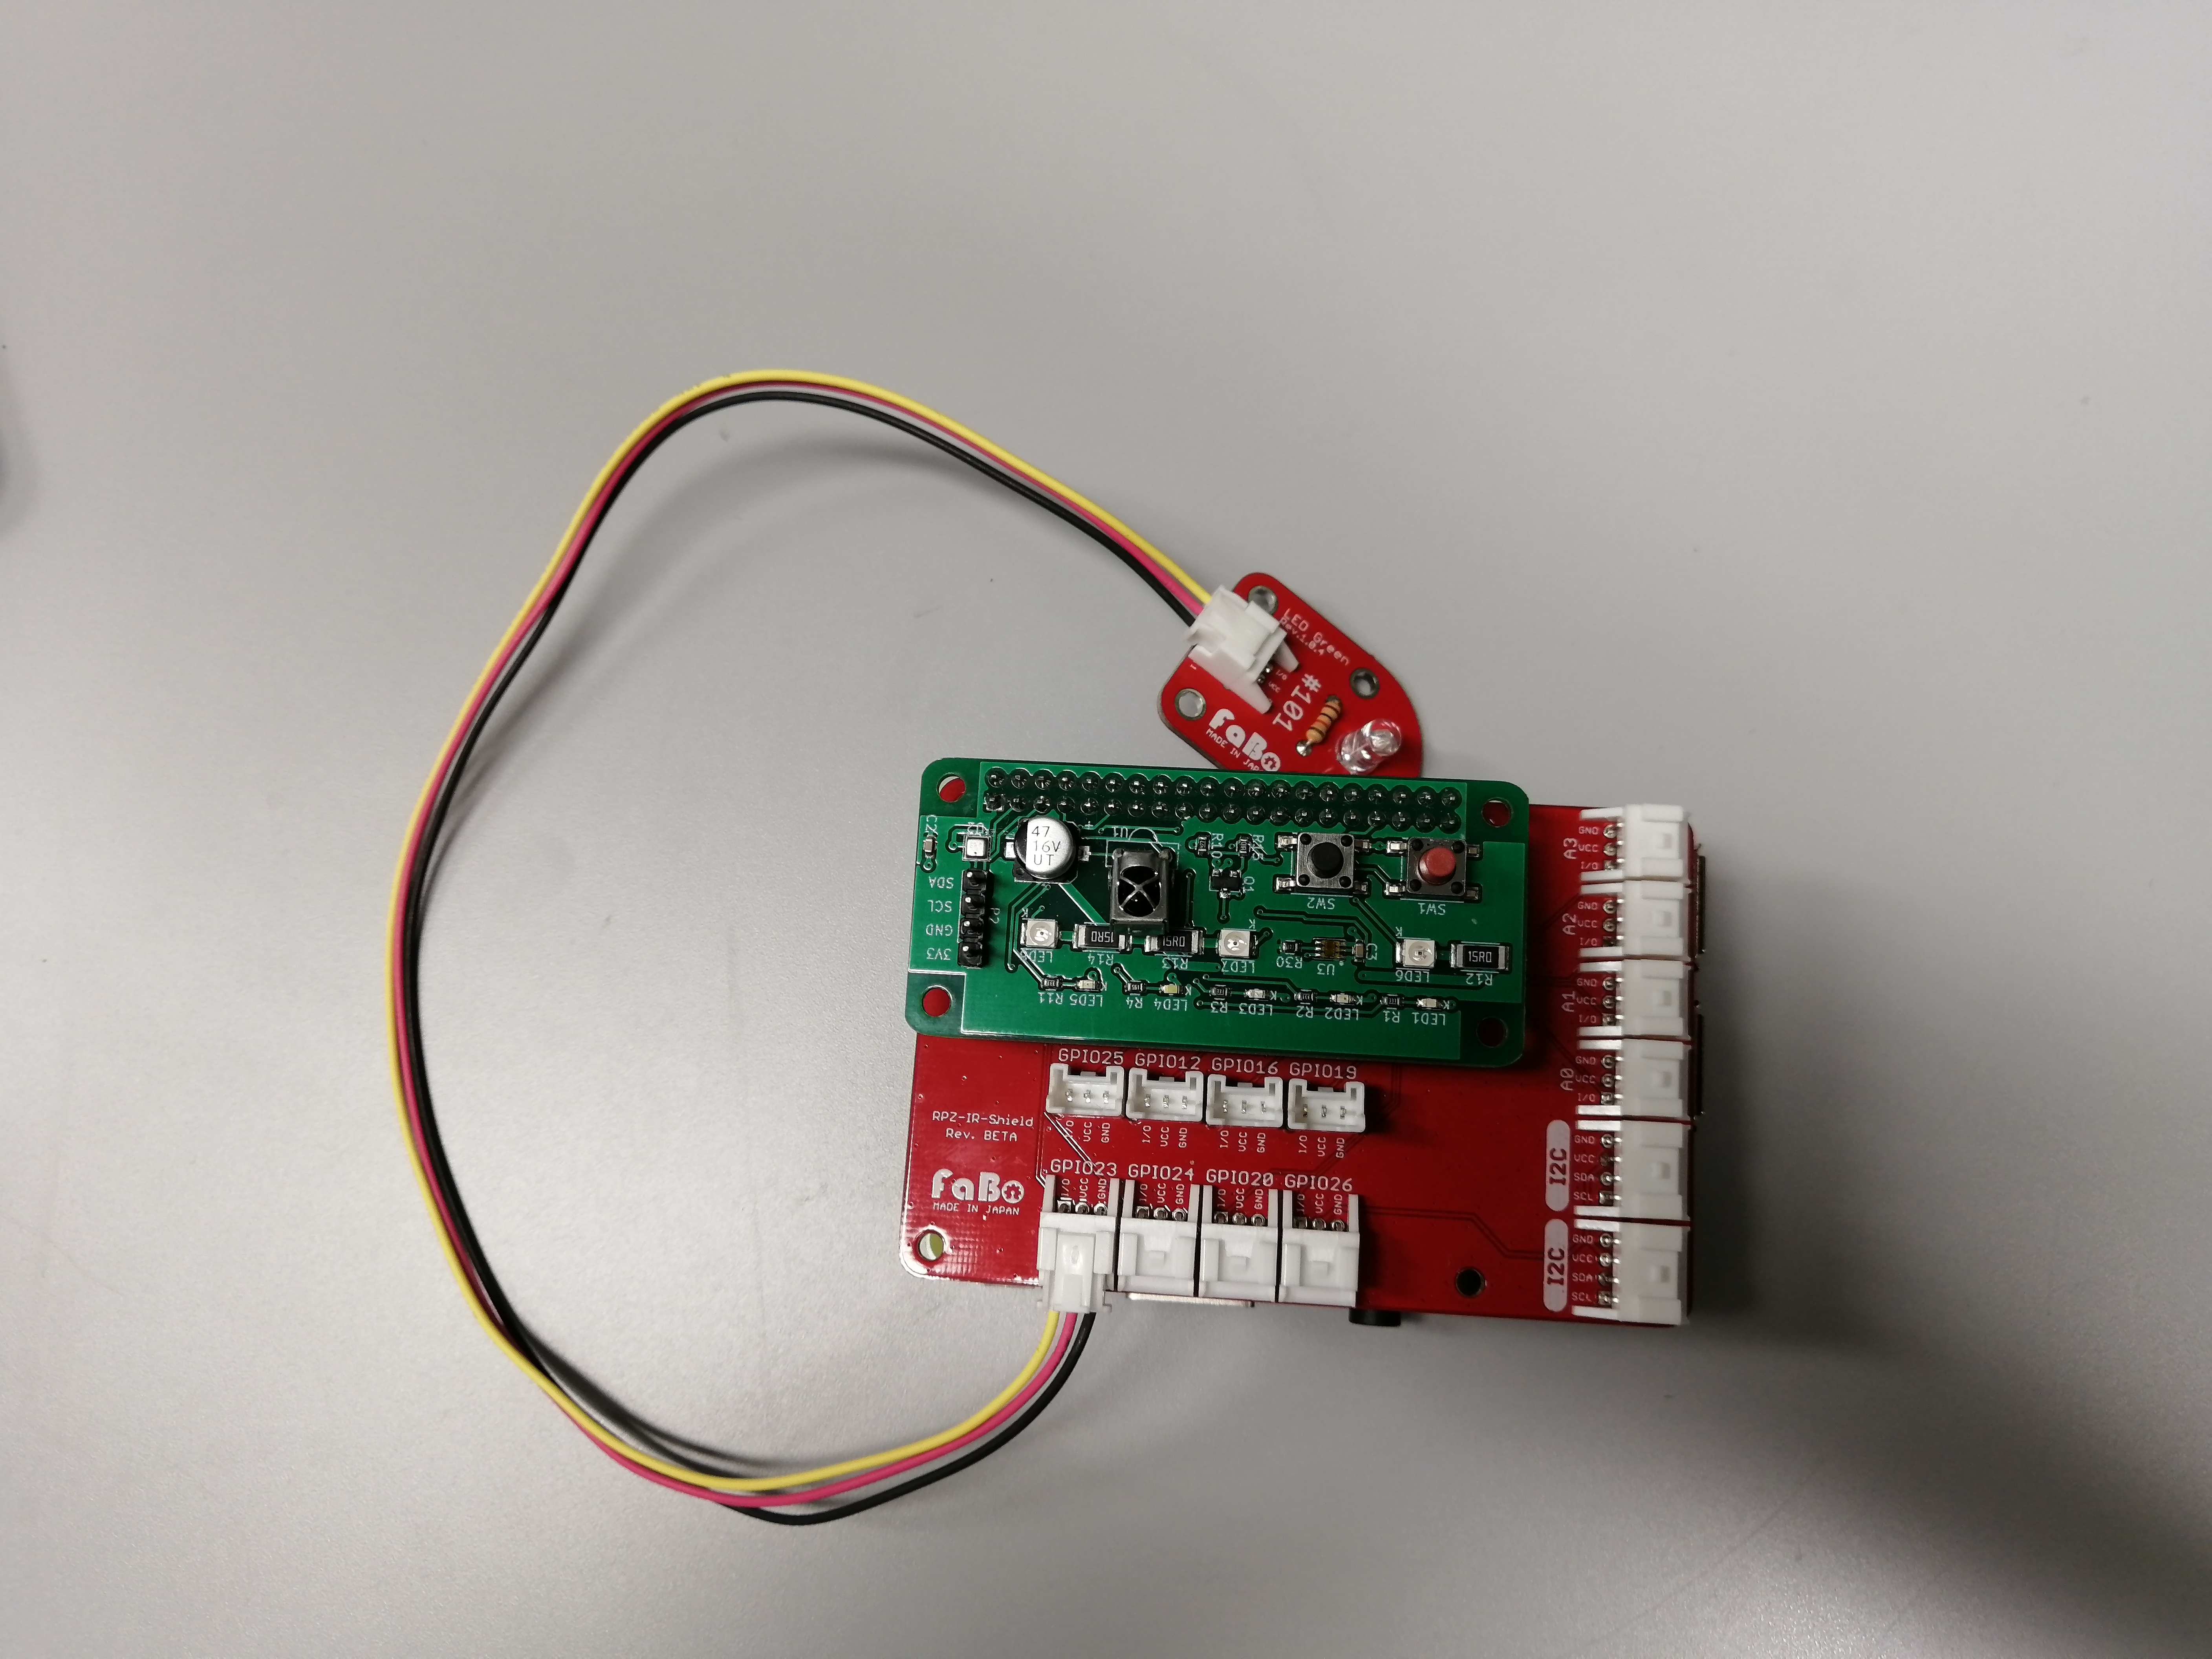
\includegraphics[width=\hsize/2]{images/chap05/text05-img009.jpg}
 \caption{シールドとケーブルのせつぞく}
\end{figure}
\item ケーブルを外す時は、とがっているツメの部分を押して引きぬいてください。ぬけない時やわからない時は周りの先生に聞いてみましょう。\\
\begin{figure}[H]
  \begin{minipage}[t]{0.48\columnwidth}
    \centering
 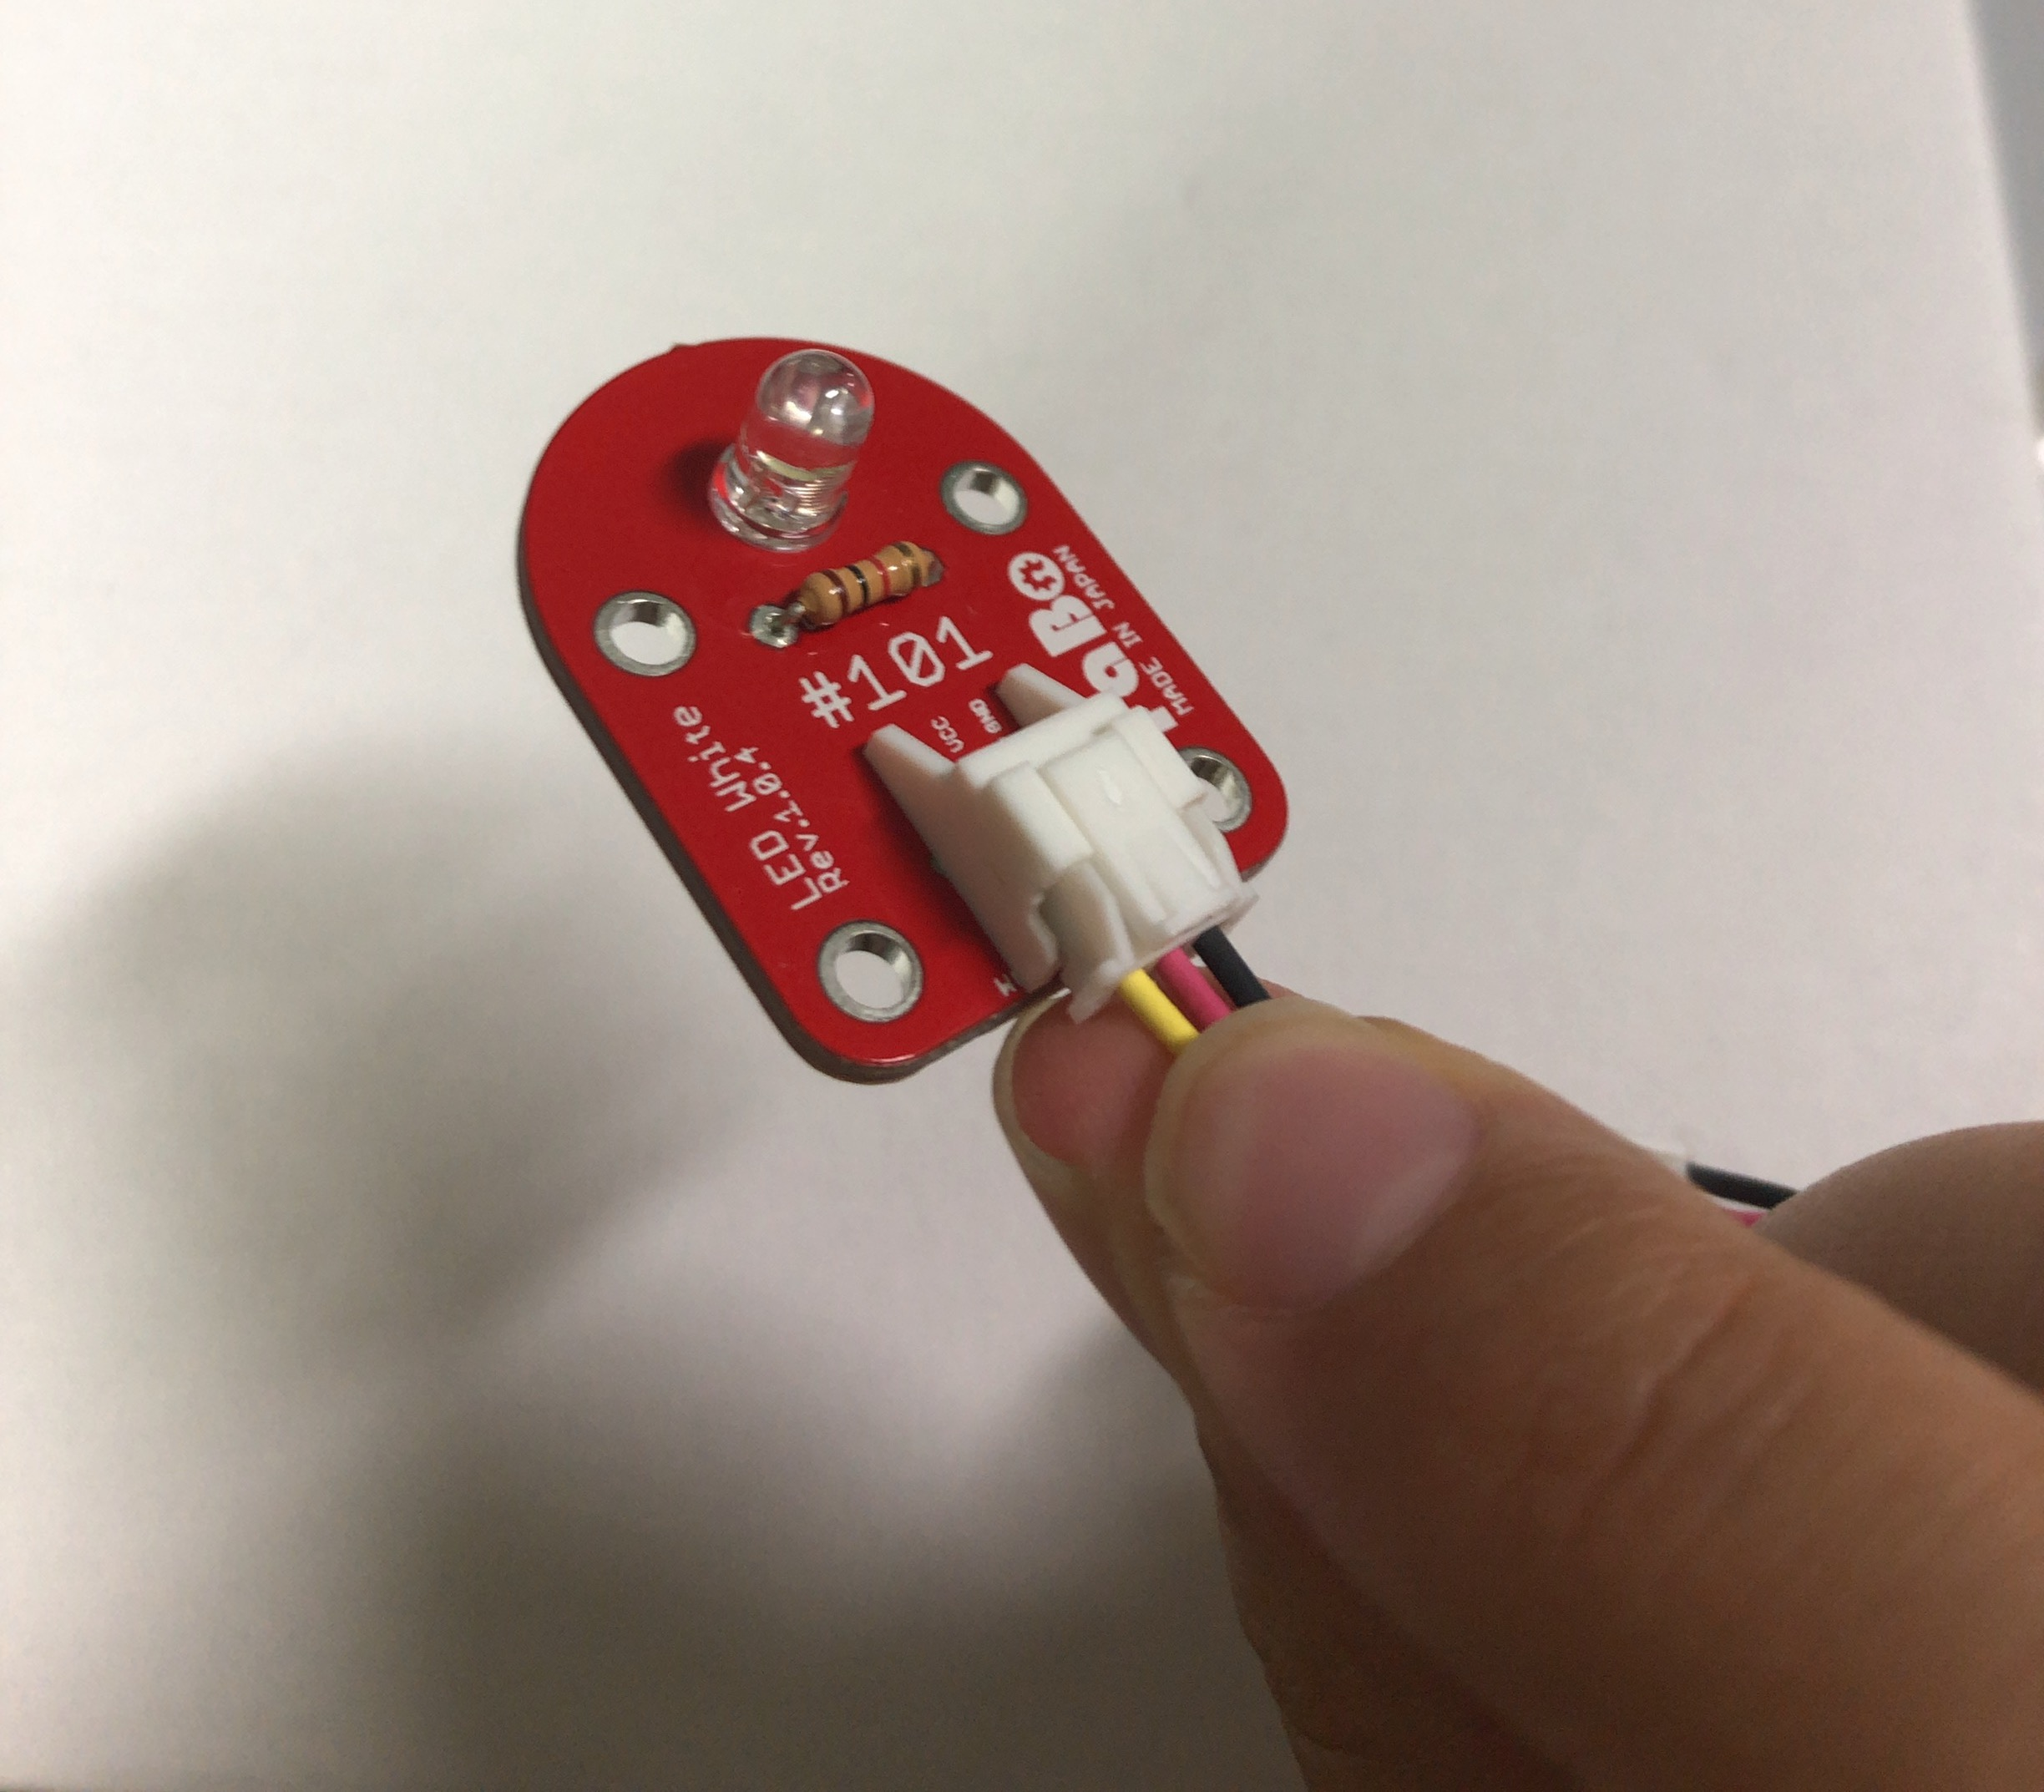
\includegraphics[width=0.8\hsize]{images/chap05/text05-img010.jpg}
    \caption{ケーブルのツメ}
白い部分の下の方を押します。
  \end{minipage}
  \hspace{0.04\columnwidth} % ここで隙間作成
  \begin{minipage}[t]{0.48\columnwidth}
    \centering
    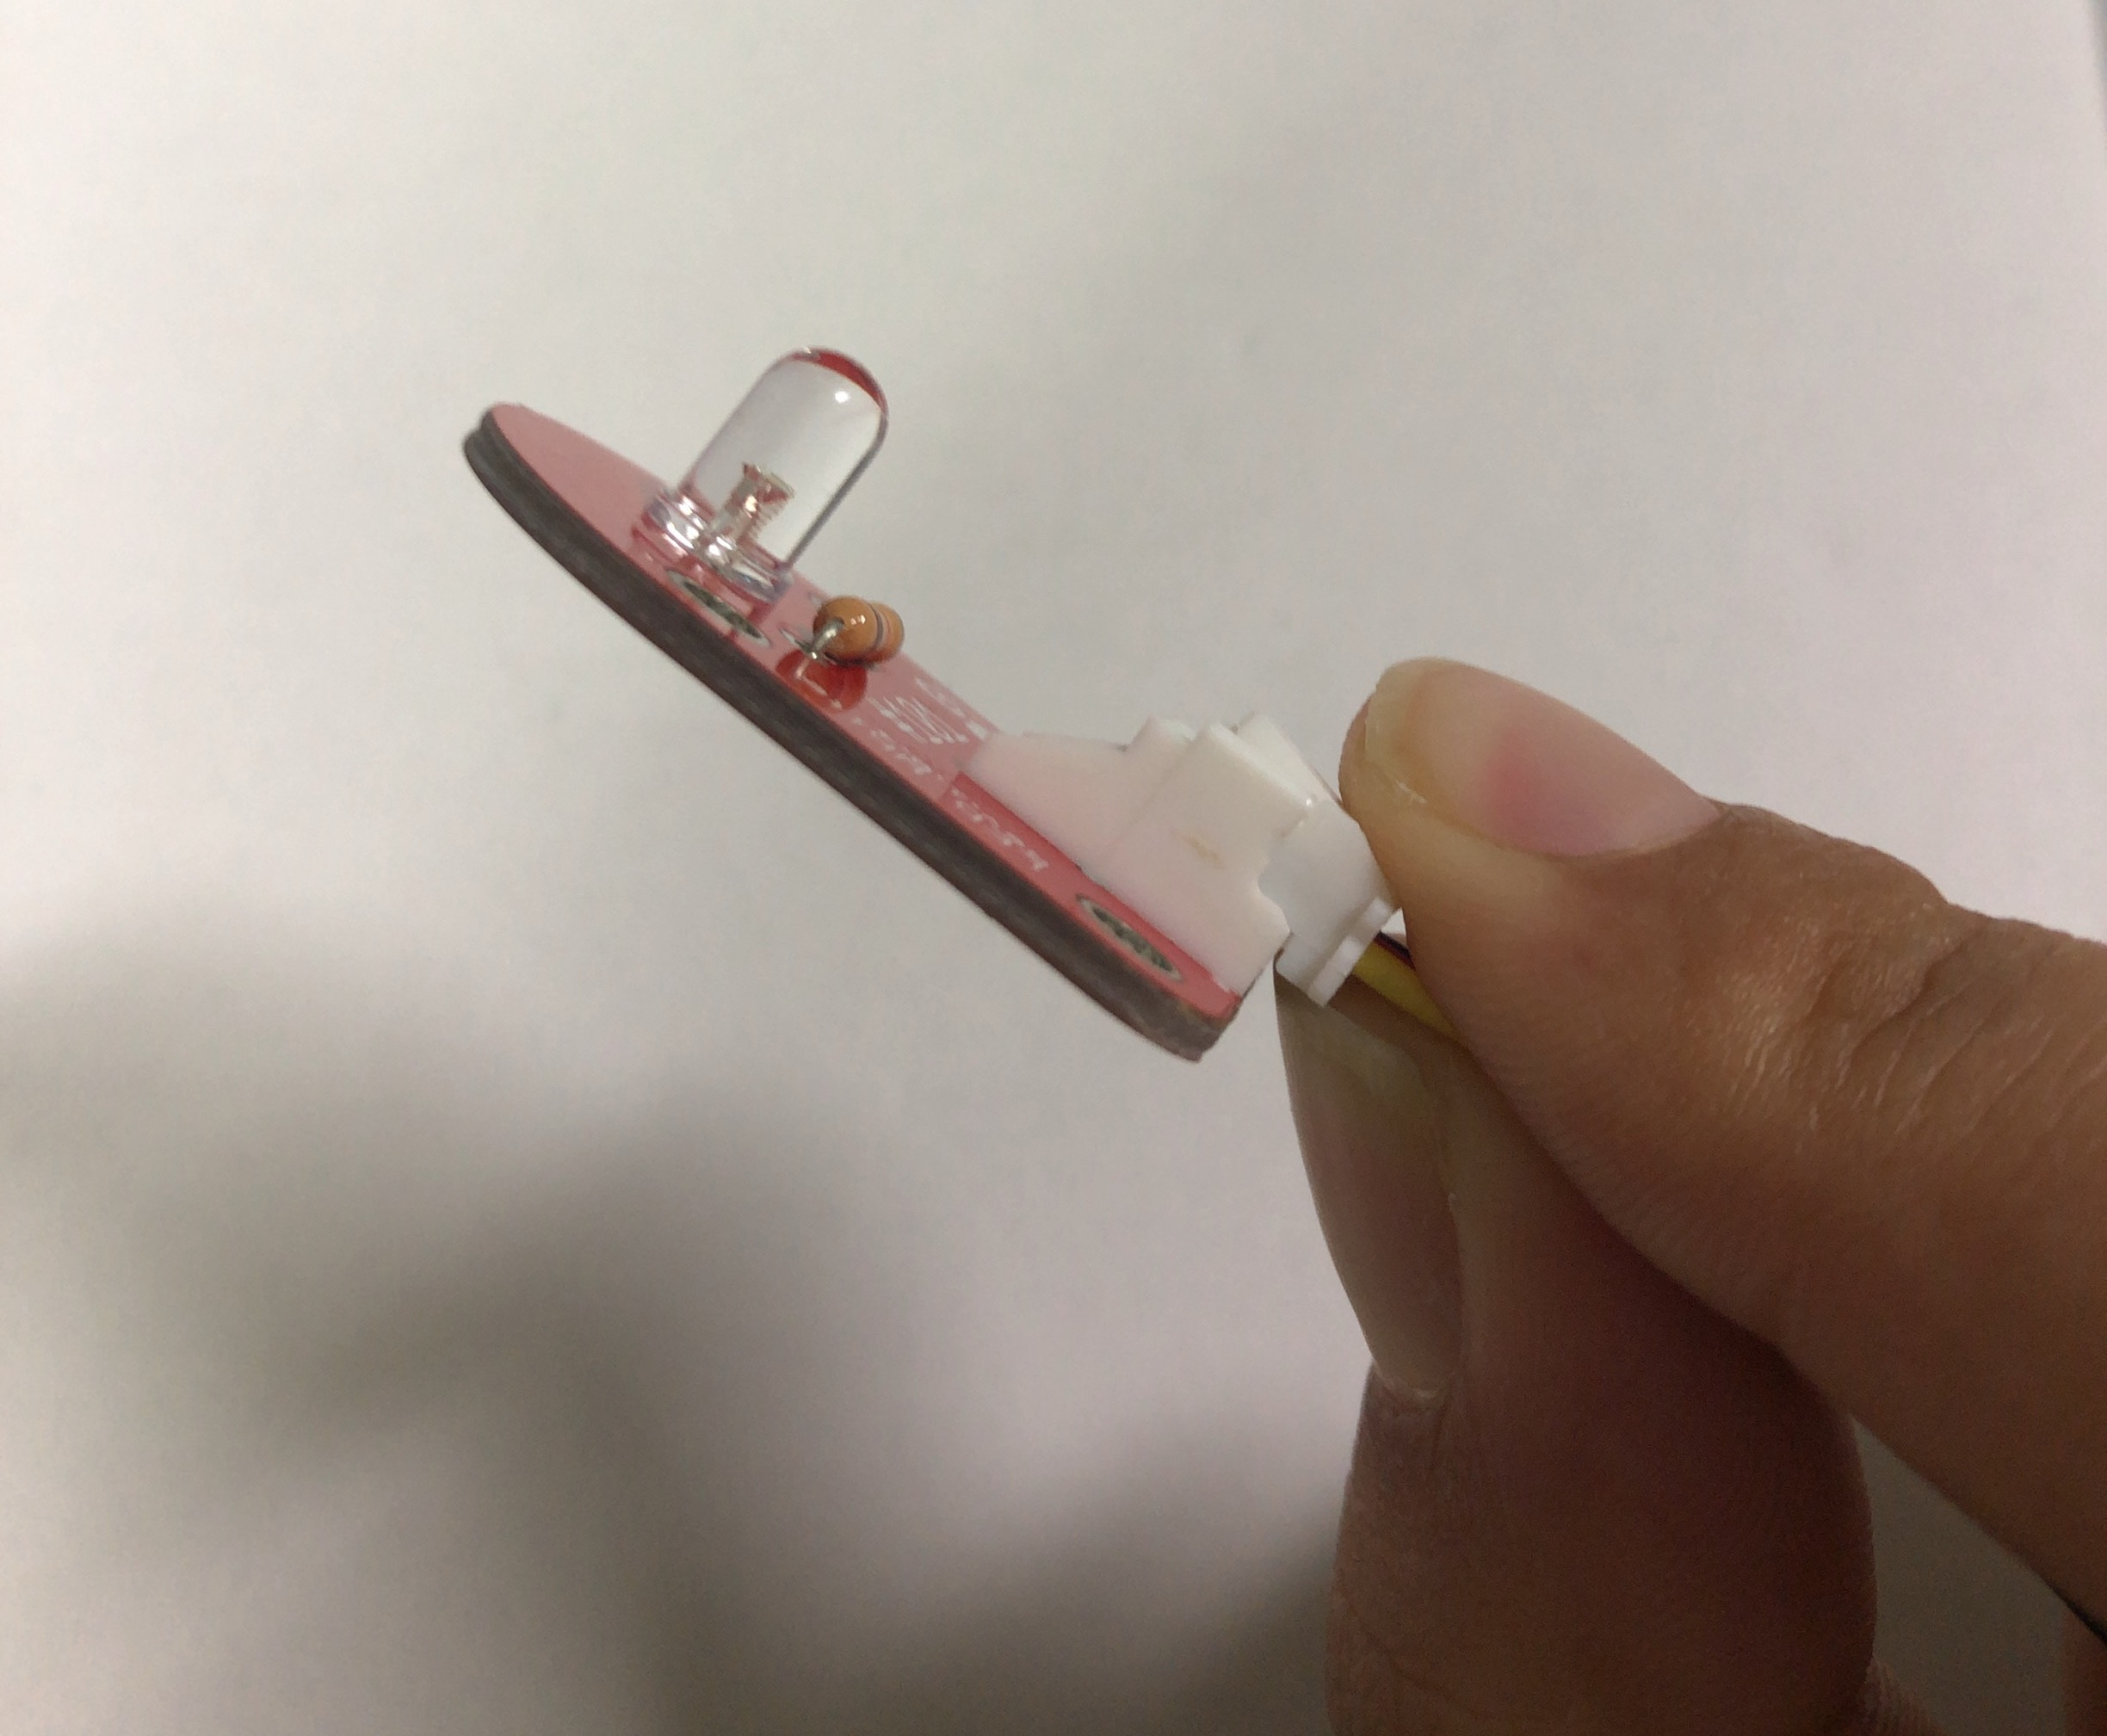
\includegraphics[width=0.8\hsize]{images/chap05/text05-img011.jpg}
    \caption{ケーブルのツメの押し方}
ツメの部分が少し浮いたら引きぬきましょう。抜けないときは無理に引っぱらず、周りの先生に聞きましょう。
  \end{minipage}
\end{figure}
\end{enumerate}
\begin{tcolorbox}[title=\useOmetoi]
\begin{enumerate}
\item Raspberry PiとLEDを上記の手順を見ながらつなげてみましょう。
\end{enumerate}
\end{tcolorbox}















